\newcommand{\bouwen}{https://woordenboek.vlaamsegebarentaal.be/gloss/BOUWEN?sid=1906}
\newcommand{\telefoneren}{https://woordenboek.vlaamsegebarentaal.be/gloss/TELEFONEREN?sid=11870}
\newcommand{\melk}{https://woordenboek.vlaamsegebarentaal.be/gloss/MELK?sid=7418}
\newcommand{\hebben}{https://woordenboek.vlaamsegebarentaal.be/gloss/HEBBEN?sid=4801}
\newcommand{\waarom}{https://woordenboek.vlaamsegebarentaal.be/gloss/WAAROM?sid=13564}
\newcommand{\haas}{https://woordenboek.vlaamsegebarentaal.be/gloss/HAAS?sid=16146}
\newcommand{\valentijn}{https://woordenboek.vlaamsegebarentaal.be/gloss/VALENTIJN?sid=16235}
\newcommand{\herfst}{https://woordenboek.vlaamsegebarentaal.be/gloss/HERFST?sid=4897}
\newcommand{\paard}{https://woordenboek.vlaamsegebarentaal.be/gloss/PAARD?sid=8880}
\newcommand{\straat}{https://woordenboek.vlaamsegebarentaal.be/gloss/STRAAT?sid=11560}
\newcommand{\voet}{https://woordenboek.vlaamsegebarentaal.be/gloss/VOET?sid=13229}
\newcommand{\krijt}{https://woordenboek.vlaamsegebarentaal.be/gloss/KRIJT?sid=6398}
\newcommand{\baas}{https://woordenboek.vlaamsegebarentaal.be/gloss/BAAS?sid=827}
\newcommand{\keuken}{https://woordenboek.vlaamsegebarentaal.be/gloss/KEUKEN?sid=5851}
\newcommand{\lasagne}{https://woordenboek.vlaamsegebarentaal.be/gloss/LASAGNE?sid=6637}
\newcommand{\sparen}{https://woordenboek.vlaamsegebarentaal.be/gloss/SPAREN?sid=11147}
\newcommand{\potlood}{https://woordenboek.vlaamsegebarentaal.be/gloss/POTLOOD?sid=9508}
\newcommand{\gras}{https://woordenboek.vlaamsegebarentaal.be/gloss/GRAS?sid=4490}
\newcommand{\links}{https://woordenboek.vlaamsegebarentaal.be/gloss/LINKS?sid=6911}
\newcommand{\kip}{https://woordenboek.vlaamsegebarentaal.be/gloss/KIP?sid=5932}
\newcommand{\vogel}{https://woordenboek.vlaamsegebarentaal.be/gloss/VOGEL?sid=13258}
\newcommand{\kompas}{https://woordenboek.vlaamsegebarentaal.be/gloss/KOMPAS?sid=6212}
\newcommand{\batman}{https://woordenboek.vlaamsegebarentaal.be/gloss/BATMAN?sid=15821}
\newcommand{\wonen}{https://woordenboek.vlaamsegebarentaal.be/gloss/WONEN?sid=14127}
\newcommand{\leeuw}{https://woordenboek.vlaamsegebarentaal.be/gloss/LEEUW?sid=6690}
\newcommand{\opstaan}{https://woordenboek.vlaamsegebarentaal.be/gloss/OPSTAAN?sid=8682}
\newcommand{\rechts}{https://woordenboek.vlaamsegebarentaal.be/gloss/RECHTS?sid=9803}
\newcommand{\kuisen}{https://woordenboek.vlaamsegebarentaal.be/gloss/KUISEN?sid=6464}
\newcommand{\hoofd}{https://woordenboek.vlaamsegebarentaal.be/gloss/HOOFD?sid=5069}
\newcommand{\europa}{https://woordenboek.vlaamsegebarentaal.be/gloss/EUROPA?sid=3646}

\begin{figure}
    \centering
    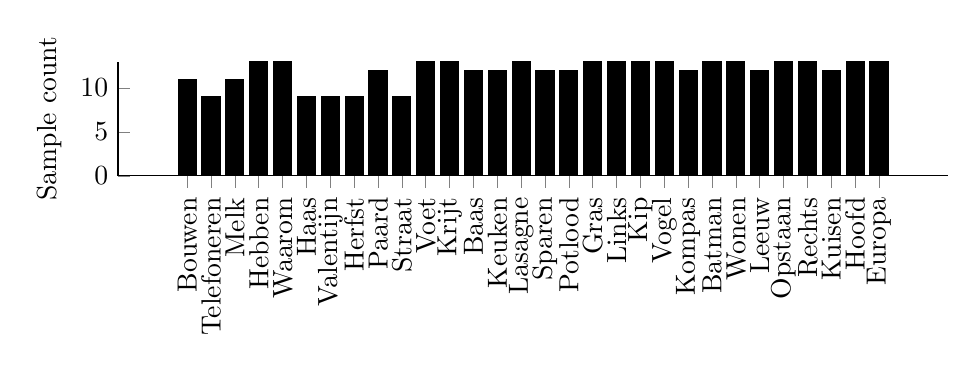
\begin{tikzpicture}
        \begin{axis}[
            ybar,
            width=\textwidth,
            height=0.25\textwidth,
            symbolic x coords={Bouwen, Telefoneren, Melk, Hebben, Waarom, Haas, Valentijn, Herfst, Paard, Straat, Voet, Krijt, Baas, Keuken, Lasagne, Sparen, Potlood, Gras, Links, Kip, Vogel, Kompas, Batman, Wonen, Leeuw, Opstaan, Rechts, Kuisen, Hoofd, Europa},
            xtick=data,
            nodes near coords={},
            ymin=0,
            ymax=13,
            axis y line*=left,
            axis x line*=bottom,
            xticklabel style={rotate=90, anchor=east},
            ylabel = {Sample count}
        ]
            % Add bars with hyperlinks
            \addplot [
                ybar,
                bar width=0.23cm,
                draw=black,
                fill=black,
                % enlarge x limits=0.2
                % xticklabel style={rotate=90, anchor=east}
            ] coordinates {(Bouwen, 11) (Telefoneren, 9) (Melk, 11) (Hebben, 13) (Waarom,13) (Haas,9) (Valentijn, 9) (Herfst,9) (Paard,12) (Straat, 9) (Voet, 13) (Krijt, 13) (Baas, 12) (Keuken, 12) (Lasagne, 13) (Sparen, 12) (Potlood, 12) (Gras, 13) (Links, 13) (Kip, 13) (Vogel, 13) (Kompas, 12) (Batman, 13) (Wonen, 13) (Leeuw, 12) (Opstaan,13) (Rechts, 13) (Kuisen, 12) (Hoofd, 13) (Europa,13)};
            
            
            \node [anchor=north] at (axis cs:Bouwen,0) {\href{\bouwen}{\rotatebox{90}{\phantom{Bouwen}}}};
            \node [anchor=north] at (axis cs:Telefoneren,0) {\href{\telefoneren}{\rotatebox{90}{\phantom{Telefoneren}}}};
            \node [anchor=north] at (axis cs:Melk,0) {\href{\melk}{\rotatebox{90}{\phantom{Melk}}}};
            \node [anchor=north] at (axis cs:Hebben,0) {\href{\hebben}{\rotatebox{90}{\phantom{Hebben}}}};
            \node [anchor=north] at (axis cs:Waarom,0) {\href{\waarom}{\rotatebox{90}{\phantom{Waarom}}}};
            \node [anchor=north] at (axis cs:Haas,0) {\href{\haas}{\rotatebox{90}{\phantom{Haas}}}};
            \node [anchor=north] at (axis cs:Valentijn,0) {\href{\valentijn}{\rotatebox{90}{\phantom{Valentijn}}}};
            \node [anchor=north] at (axis cs:Herfst,0) {\href{\herfst}{\rotatebox{90}{\phantom{Herfst}}}};
            \node [anchor=north] at (axis cs:Paard,0) {\href{\paard}{\rotatebox{90}{\phantom{Paard}}}};
            \node [anchor=north] at (axis cs:Straat,0) {\href{\straat}{\rotatebox{90}{\phantom{Straat}}}};
            \node [anchor=north] at (axis cs:Voet,0) {\href{\voet}{\rotatebox{90}{\phantom{Voet}}}};
            \node [anchor=north] at (axis cs:Krijt,0) {\href{\krijt}{\rotatebox{90}{\phantom{Krijt}}}};
            \node [anchor=north] at (axis cs:Baas,0) {\href{\baas}{\rotatebox{90}{\phantom{Baas}}}};
            \node [anchor=north] at (axis cs:Keuken,0) {\href{\keuken}{\rotatebox{90}{\phantom{Keuken}}}};
            \node [anchor=north] at (axis cs:Lasagne,0) {\href{\lasagne}{\rotatebox{90}{\phantom{Lasagne}}}};
            \node [anchor=north] at (axis cs:Sparen,0) {\href{\sparen}{\rotatebox{90}{\phantom{Sparen}}}};
            \node [anchor=north] at (axis cs:Potlood,0) {\href{\potlood}{\rotatebox{90}{\phantom{Potlood}}}};
            \node [anchor=north] at (axis cs:Gras,0) {\href{\gras}{\rotatebox{90}{\phantom{Gras}}}};
            \node [anchor=north] at (axis cs:Links,0) {\href{\links}{\rotatebox{90}{\phantom{Links}}}};
            \node [anchor=north] at (axis cs:Kip,0) {\href{\kip}{\rotatebox{90}{\phantom{Kip}}}};
            \node [anchor=north] at (axis cs:Vogel,0) {\href{\vogel}{\rotatebox{90}{\phantom{Vogel}}}};
            \node [anchor=north] at (axis cs:Kompas,0) {\href{\kompas}{\rotatebox{90}{\phantom{Kompas}}}};
            \node [anchor=north] at (axis cs:Batman,0) {\href{\batman}{\rotatebox{90}{\phantom{Batman}}}};
            \node [anchor=north] at (axis cs:Wonen,0) {\href{\wonen}{\rotatebox{90}{\phantom{Wonen}}}};
            \node [anchor=north] at (axis cs:Leeuw,0) {\href{\leeuw}{\rotatebox{90}{\phantom{Leeuw}}}};
            \node [anchor=north] at (axis cs:Opstaan,0) {\href{\opstaan}{\rotatebox{90}{\phantom{Opstaan}}}};
            \node [anchor=north] at (axis cs:Rechts,0) {\href{\rechts}{\rotatebox{90}{\phantom{Rechts}}}};
            \node [anchor=north] at (axis cs:Kuisen,0) {\href{\kuisen}{\rotatebox{90}{\phantom{Kuisen}}}};
            \node [anchor=north] at (axis cs:Hoofd,0) {\href{\hoofd}{\rotatebox{90}{\phantom{Hoofd}}}};
            \node [anchor=north] at (axis cs:Europa,0) {\href{\europa}{\rotatebox{90}{\phantom{Europa}}}};
        \end{axis}
    \end{tikzpicture}
    \caption{The number of dictionary queries per gloss is distributed approximately uniformly
    with mean 11.93. Each label on the horizontal axis is a link to the corresponding video within the Flemish Sign Language dictionary.}
    \label{fig:frequency}
\end{figure}